\section{Lesson 05 --- 15/10/2026}

\subsection{Eager learners}
Differently from lazy learners, \g{eager} learners, when given a set of training data, construct a generalization model before receiving new data to classify. We need to build our own classifier and then evaluate whether it performs well or not. To evaluate its performance we need a ground truth that is similar to the training set in structure (it needs to have the class label), but different in values: the \g{test set}. To evaluate the classifier we need a metric. One option is the \g{accuracy}, which measures the percentage of test set instances that are correctly classified. This metric is not always a good choice when the classes are highly unbalanced.

Another frequent problem in classification is \g{overtraining} (overfitting). We have overtraining when the classifier fits the training data too closely, including noise and dataset-specific peculiarities, and therefore performs worse on unseen data. This can happen, for example, when the two classes are not well separated and overlap, possibly also because of noise. If there is overtraining, the classifier is too tuned on the training set and is not able to generalize well. To detect it we can first classify the instances in the training set, then the instances in the test set, and compare the two accuracies. If the test accuracy is much lower than the training accuracy, the classifier is likely overtrained; if the two accuracies are close, the classifier is generalizing well.

\subsection{Linear support vector machine}

A linear \g{support vector machine} (SVM) is a simple model that looks for a linear separator (a line) in the data. There could be an infinite number of lines that separate our data, but we want to find the ``best'' one, the one with the lowest classification error on unseen data. In higher dimensions we will use hyperplanes instead of lines, so from now on we use this term to refer to the decision boundary. In an SVM we look for the \g{maximum margin hyperplane} (MMH). By margin we mean the distance between the hyperplane and the closest sample of either class: the two \s{sides} of the margin are parallel to the hyperplane and at the same distance from it. Intuitively, a hyperplane with a larger margin should be more accurate on future data than one with a smaller margin.

\begin{center}
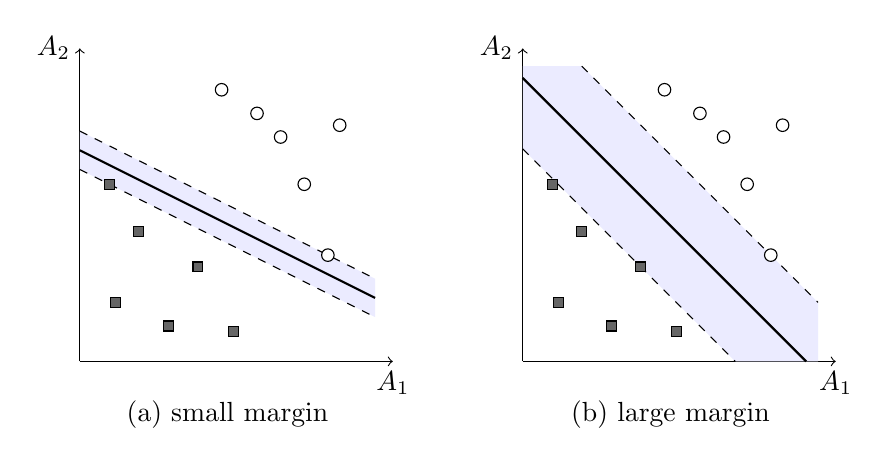
\begin{tikzpicture}[scale=0.75,
    possample/.style={circle, draw, fill=white, inner sep=1.6pt},
    negsample/.style={rectangle, draw, fill=black!60, inner sep=1.8pt}]
  % (a) small margin
  \begin{scope}
    \draw[->] (0,0) -- (5.3,0) node[below] {$A_1$};
    \draw[->] (0,0) -- (0,5.3) node[left] {$A_2$};
    \fill[blue!8] (0,3.25) -- (5,0.75) -- (5,1.4) -- (0,3.9) -- cycle;
    \draw[dashed] (0,3.25) -- (5,0.75);
    \draw[dashed] (0,3.9) -- (5,1.4);
    \draw[thick] (0,3.575) -- (5,1.075);
    \foreach \p in {(0.6,1.0),(1.0,2.2),(1.5,0.6),(2.0,1.6),(0.5,3.0),(2.6,0.5)} \node[negsample] at \p {};
    \foreach \p in {(3.0,4.2),(3.8,3.0),(4.4,4.0),(2.4,4.6),(4.2,1.8),(3.4,3.8)} \node[possample] at \p {};
    \node at (2.5,-0.9) {(a) small margin};
  \end{scope}
  % (b) large margin
  \begin{scope}[xshift=7.5cm]
    \draw[->] (0,0) -- (5.3,0) node[below] {$A_1$};
    \draw[->] (0,0) -- (0,5.3) node[left] {$A_2$};
    \fill[blue!8] (0,3.6) -- (3.6,0) -- (5,0) -- (5,1) -- (1,5) -- (0,5) -- cycle;
    \draw[dashed] (0,3.6) -- (3.6,0);
    \draw[dashed] (1,5) -- (5,1);
    \draw[thick] (0,4.8) -- (4.8,0);
    \foreach \p in {(0.6,1.0),(1.0,2.2),(1.5,0.6),(2.0,1.6),(0.5,3.0),(2.6,0.5)} \node[negsample] at \p {};
    \foreach \p in {(3.0,4.2),(3.8,3.0),(4.4,4.0),(2.4,4.6),(4.2,1.8),(3.4,3.8)} \node[possample] at \p {};
    \node at (2.5,-0.9) {(b) large margin};
  \end{scope}
\end{tikzpicture}
\end{center}

Both hyperplanes in the figure correctly classify all the training samples, but we prefer (b) because its margin is larger. To find the MMH we need to describe hyperplanes and margins with formulas. Let the training set be $(x_1, y_1), \dots, (x_n, y_n)$, where $x_i \in \R^d$ is a sample and $y_i \in \{+1, -1\}$ is its class label. A separating hyperplane is a linear classifier and can be written as
\[
  H: \ w^T x + b = 0,
\]
where $w = [w_1 \ \cdots \ w_d]^T$ is a weight vector and $b$ is a scalar called \s{bias}. With two attributes this is just the line $b + w_1 x_1 + w_2 x_2 = 0$. Any point above the hyperplane satisfies $w^T x + b > 0$, and any point below it satisfies $w^T x + b < 0$. So the classifier is simply the sign of $w^T x + b$.

Now we describe the two sides of the margin. They are two hyperplanes parallel to $H$, so they have the form $w^T x + b = \pm c$ for some $c > 0$. Since $w$ and $b$ can be multiplied by the same positive constant without changing the separating hyperplane, we can choose a canonical scaling such that $c = 1$, so the two sides of the margin are
\[
  H_1: \ w^T x + b = +1, \qquad H_2: \ w^T x + b = -1.
\]
Requiring that every sample lies on the correct side of its margin side gives
\[
  w^T x_i + b \ge +1 \quad \text{if } y_i = +1, \qquad
  w^T x_i + b \le -1 \quad \text{if } y_i = -1,
\]
which can be combined into a single constraint
\[
  y_i\,(w^T x_i + b) \ge 1 \quad \text{for all } i.
\]
The samples lying on $H_1$ or $H_2$ satisfy the constraint with equality, $y_i\,(w^T x_i + b) = 1$: these are the \g{support vectors}. They are the samples closest to the separating hyperplane, the most difficult to classify, and they are the only ones that define the final classifier.

The margin can now be written only in terms of $w$. The distance of a point $x$ from the hyperplane $H$ is
\[
  \operatorname{dist}(x, H) = \frac{|w^T x + b|}{\norm{w}}.
\]
For a support vector the numerator is $1$, so each side of the margin is at distance $1/\norm{w}$ from $H$. Hence the margin is
\[
  \rho = \frac{2}{\norm{w}}.
\]
Maximizing the margin is therefore equivalent to minimizing $\norm{w}$. For mathematical convenience we minimize $\frac{1}{2}\norm{w}^2$, which has the same minimizer, and we obtain the optimization problem
\[
  \min_{w,b} \ \frac{1}{2}\norm{w}^2 \quad \text{subject to } y_i\,(w^T x_i + b) \ge 1, \quad i = 1, \dots, n.
\]
The constraints enforce correct separation, while the objective selects, among all feasible separators, the one with maximum margin.

We can solve it using Lagrange multipliers and the dual problem, which gives a maximization problem that reveals which samples become support vectors ($\alpha_i > 0 \iff x_i$ is a support vector). To predict the class of a new sample $x$ we compute the inner products with the support vectors only:
\[
  f(x) = \operatorname{sign}\Bigl(\sum_{i} \alpha_i y_i\, x_i^T x + b\Bigr).
\]
If the result is positive, the sample is above the separator and is assigned to class $+1$, otherwise to class $-1$.

\subsection{Nonlinear SVM and the kernel idea}

The problem with SVM is that it is not always possible to linearly separate the classes, and in that case the optimization problem has no solution. To solve this problem we can apply a nonlinear mapping function $\Phi: x \to \varphi(x)$ to transform the data into a higher-dimensional space. This transformation is made easier by exploiting the \g{kernel function}. A kernel function is a function that is equivalent to an inner product in some feature space, $K(x_i, x_j) = \varphi(x_i)^T \varphi(x_j)$: it implicitly maps data to a high-dimensional space.

\begin{example}
Consider 2-dimensional vectors $x = [x_1 \ x_2]^T$ and let $K(x_i, x_j) = (1 + x_i^T x_j)^2$. We need to show that $K(x_i, x_j) = \varphi(x_i)^T \varphi(x_j)$:
\begin{align*}
  K(x_i, x_j) &= (1 + x_i^T x_j)^2 \\
  &= 1 + x_{i1}^2 x_{j1}^2 + 2\, x_{i1} x_{j1} x_{i2} x_{j2} + x_{i2}^2 x_{j2}^2 + 2\, x_{i1} x_{j1} + 2\, x_{i2} x_{j2} \\
  &= \bigl[1 \ \ x_{i1}^2 \ \ \sqrt{2}\, x_{i1} x_{i2} \ \ x_{i2}^2 \ \ \sqrt{2}\, x_{i1} \ \ \sqrt{2}\, x_{i2}\bigr]
     \bigl[1 \ \ x_{j1}^2 \ \ \sqrt{2}\, x_{j1} x_{j2} \ \ x_{j2}^2 \ \ \sqrt{2}\, x_{j1} \ \ \sqrt{2}\, x_{j2}\bigr]^T \\
  &= \varphi(x_i)^T \varphi(x_j),
\end{align*}
where $\varphi(x) = \bigl[1 \ \ x_1^2 \ \ \sqrt{2}\, x_1 x_2 \ \ x_2^2 \ \ \sqrt{2}\, x_1 \ \ \sqrt{2}\, x_2\bigr]^T$.
\end{example}

Some popular kernel functions are:
\begin{itemize}
  \item \g{Linear}: $K(x_i, x_j) = x_i^T x_j$;
  \item \g{Polynomial} of power $p$: $K(x_i, x_j) = (1 + x_i^T x_j)^p$;
  \item \g{Gaussian} (radial-basis function): $K(x_i, x_j) = e^{-\frac{\norm{x_i - x_j}^2}{2\sigma^2}}$.
\end{itemize}

What happens if we have more than two classes? The standard SVM is naturally binary. To apply it to more than two classes we can follow the \g{one-vs-rest} strategy: we decompose the problem into identifying one single class against all the others, and we repeat this for every class. To classify new instances we choose the class with the highest score (we cannot use the sign as before, because we could have more than one positive result).

\subsection{Decision tree}

Another model we will see is the \g{decision tree}. This model is still widely used today because it is considered one of the most interpretable classifiers. This means that the classifier itself is able to explain how the given input is correlated to the output. Other very good characteristics of decision trees are: it requires no domain knowledge, it can be learned directly from the data, it can handle many attributes and there is no parameter to set. A decision tree is a flowchart-like structure where the internal \g{nodes} represent the attribute tests, the \g{branches} are the outcomes of the tests and in the \g{leaves} we find the class labels. The problem is: how can we generate the decision tree?

Of course the choice of which test to put in each node will affect the final result, so we need an algorithm to decide what to put in the nodes.

The main goal of the decision tree is to generate in the sample space some sub-spaces where there are only members of one class, so when I have to classify a new object that falls in one particular sub-space I can choose the class of that sub-space.

\subsubsection{Algorithm for decision tree induction}

Decision tree induction follows a greedy, top-down, recursive divide-and-conquer strategy:
\begin{itemize}
  \item at each stage we make the locally optimal split;
  \item we hope that these local choices lead to a good global tree;
  \item the instances start at the root and are recursively partitioned.
\end{itemize}
We assume that the attributes are categorical: continuous attributes are discretized in advance. The test attribute is selected using a heuristic or statistical measure, for example the information gain or related impurity measures. The recursion stops when all the instances at a node belong to the same class, when no attributes are left (and we use majority voting), or when no instances are left.

\begin{algorithm}[H]
  \caption{Decision tree induction}
  \KwIn{a set $D$ of training instances, a list of candidate attributes}
  \KwOut{a decision tree}
  create a node $N$ containing all the instances of $D$\;
  \uIf{all the instances in $D$ belong to the same class $C$}{
    \Return $N$ as a leaf labelled with $C$\;
  }
  \uIf{the attribute list is empty}{
    \Return $N$ as a leaf labelled with the majority class in $D$\;
  }
  select the best test attribute $A$ using the selection measure\;
  label $N$ with $A$ and remove $A$ from the attribute list\;
  \ForEach{outcome $a_j$ of $A$}{
    let $D_j$ be the subset of instances in $D$ with outcome $a_j$\;
    \eIf{$D_j$ is empty}{
      attach to $N$ a leaf labelled with the majority class in $D$\;
    }{
      attach to $N$ the tree returned by the algorithm applied to $D_j$\;
    }
  }
  \Return $N$\;
\end{algorithm}
